\documentclass[11pt,a4paper]{article}

\usepackage[margin=25mm]{geometry}
\usepackage[T1]{fontenc}
\usepackage{lmodern}
\usepackage{amsmath,amssymb}
\usepackage{siunitx}            % \SI{240}{\volt}, \ang{120}
\usepackage{graphicx}
\usepackage{booktabs,tabularx}
\usepackage{enumitem}
\usepackage{xcolor}
\usepackage{siunitx}
\usepackage[numbers]{natbib}
\usepackage[colorlinks=true,linkcolor=black,citecolor=black,urlcolor=blue]{hyperref}
\usepackage[capitalise,noabbrev]{cleveref}

% Planning notes: grey, small. Delete each one as you replace it with text.
\newcommand{\plan}[1]{\par{\small\color{gray}\itshape #1}\par}
% Status line under each section title.
\newcommand{\status}[1]{{\small\color{orange!80!black}\textsc{Status:} #1}\par\medskip}
% Phasor in polar form, e.g. \ph{120}{0} -> 120 angle 0 degrees.
\newcommand{\ph}[2]{#1\,\angle\,#2^{\circ}}

\title{Beyond the Orange Wire\\[4pt]
  \large Designing, Loading and Troubleshooting High-Leg and Open-Delta Services}
\author{Shankar Ramharack}
\date{Application note OW-AN 001 \quad Edition 0.1 (draft) \quad \today}

\begin{document}
\maketitle

\begin{abstract}
An open application note on 120/240\,V four-wire delta services: the closed (high-leg) delta and the open delta. It sets out one design method for both, answers the ``208\,V question'' with evidence, catalogues common field problems, and works two examples designed from scratch: a casual-dining restaurant and a \SI{250}{m^3/day} seawater reverse-osmosis plant. NEC 2023 is the reference code; every citation is logged in \cref{app:verification}.
\end{abstract}

\tableofcontents
\clearpage

% =====================================================================
\section*{Preface}
\addcontentsline{toc}{section}{Preface}
\status{outline}
\plan{Who this is for: practising designers and field engineers first; students second, with full derivations in \cref{sec:phasors} and \cref{app:notation}.}
\plan{What makes it different: one method for closed and open delta; quantified shortcut errors; an evidence-based answer to the 208\,V question; two worked examples; everything reproducible.}
\plan{Conventions: NEC 2023 \citep{nfpa70_2023} as ``NEC 2023 xxx.xx''; 120/240\,V, 60\,Hz unless stated; high leg is phase B throughout.}

% =====================================================================
% PART I: FOUNDATIONS
% =====================================================================
\section{What a four-wire delta is, and when to use it}\label{sec:what-when}
\status{outline, drafting in v0.1}

\subsection{The three services you will meet}
\plan{120/208Y as the reference; 120/240\,V closed (high-leg) delta; 120/240\,V open delta; 240\,V three-wire delta for context.}
\subsection{Where the high leg comes from}
\plan{Centre-tapped lighting transformer and the neutral; why one phase sits at about 208\,V to neutral (derived in \cref{sec:phasors}); trade names; orange marking.}
\subsection{Prior work}
\plan{Kersting's IEEE Transactions on Industry Applications papers on four-wire delta banks; the IEEE Four-Wire Delta Test Feeder; what this note adds.}
\subsection{Where you still find it}
\plan{Legacy utility practice; light industrial and rural services; motor-heavy loads with little 120\,V load; Caribbean utilities (\cref{sec:caribbean}).}
\subsection{Choosing between four-wire delta and 120/208Y}
\plan{Decision table: motor vs 120\,V load share; 240\,V vs 208\,V equipment; what the utility offers; PV and battery inverters; generators and transfer switches; panelboard and breaker availability; risk of conversion to wye; labelling risk.}
\subsection{When open delta makes sense}
\subsection{What this note does not cover}

% ---------------------------------------------------------------------
\section{High-leg nuances and NEC 2023 requirements}\label{sec:nec}
\status{outline, drafting in v0.1}
\plan{Every section number below is a candidate until checked against the NEC 2023 text and logged in \cref{app:verification}.}

\subsection{Identifying the high leg}
\plan{Conductor marking (candidate 110.15); services (230.56); feeder and branch identification (215.12, 210.5).}
\subsection{Panelboard phase arrangement}
\plan{High leg on phase B (candidate 408.3(E)(1)); the metering exception.}
\subsection{Field marking}
\plan{Caution labels (candidate 408.3(F)(1)).}
\subsection{Overcurrent devices: slash vs straight ratings}
\plan{Candidate 240.85; single-pole breakers and the B position.}
\subsection{Single-pole loads and the high leg}
\plan{What the code requires and what it does not say; full investigation in \cref{sec:208v}.}
\subsection{Grounding and bonding}
\subsection{Neutral sizing and loading}
\plan{Candidate 220.61.}
\subsection{Surge protective devices and meters}
\plan{Line-to-ground ratings (candidate Article 242).}
\subsection{Labelling and documentation checklist}

% ---------------------------------------------------------------------
\section{Phasors and the math of four-wire delta}\label{sec:phasors}
\status{outline, drafting now}

\subsection{Conventions}
\plan{Phase sequence, reference phasor, sign conventions.}

\subsection{Voltage phasors in a closed delta with a centre tap}\label{sec:voltage-phasors}
In a centre-tapped closed delta, commonly called a high-leg delta, the winding
between lines A and C is tapped at its midpoint, and the tap is grounded to form
the neutral N. On a pole-mounted bank this winding is the secondary of the
larger \emph{lighting} transformer; the two smaller \emph{power} transformers
complete the delta (\cref{fig:closed-bank}).

\begin{figure}[htbp]
  \centering
  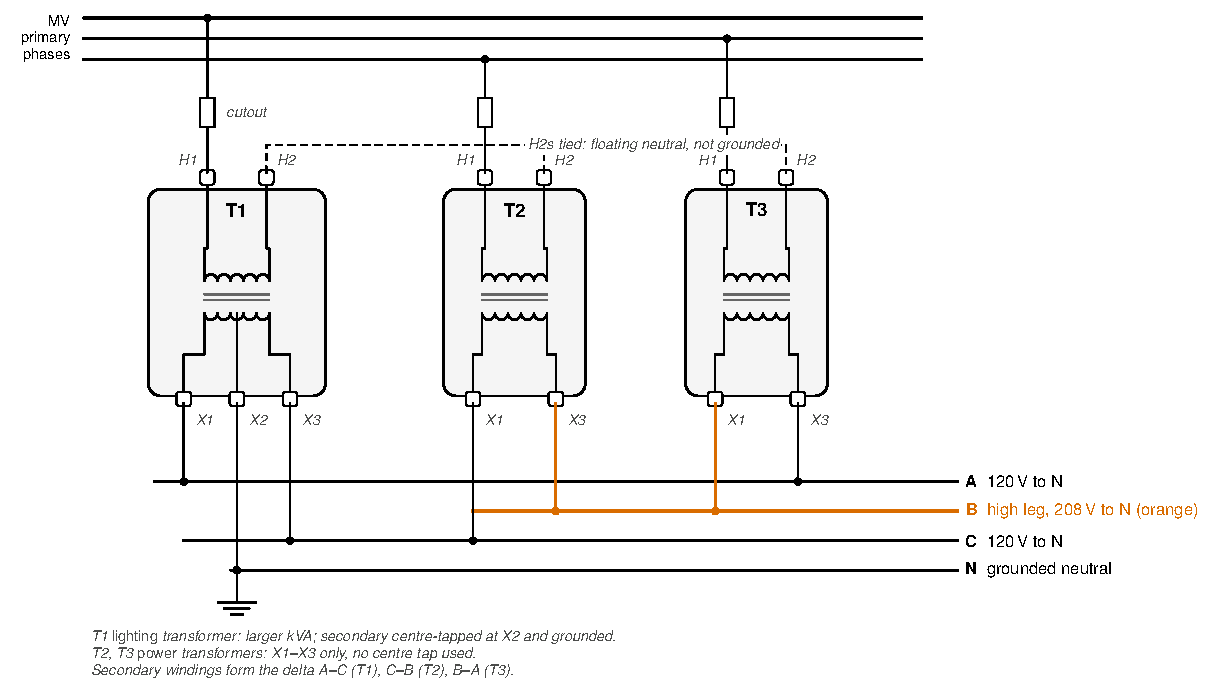
\includegraphics[width=\linewidth]{figures/fig-closed-bank.pdf}
  \caption{Closed-delta bank of three single-phase pole-mounted transformers,
    floating-wye primary, 120/240\,V four-wire delta secondary. T1, the lighting
    transformer, is centre-tapped at X2 to form the grounded neutral; B, the high
    leg, is shown in orange.}
  \label{fig:closed-bank}
\end{figure}
\plan{FUTURE FIGURE: padmount option. Draw a single three-phase padmount
transformer with a 120/240\,V four-wire delta secondary: one tank, three LV
windings inside forming the delta, one of them centre-tapped and bonded to the
neutral (X0) terminal, LV bushings in the secondary compartment, and the high
leg marked orange. Match the style and labels of \cref{fig:closed-bank} (A, B, C,
N; orange B) so the two read as a pair. Add one or two sentences on when a
padmount is used instead of a pole bank (underground and commercial services),
and note that a padmount cannot be run as an open delta. VERIFY before drawing:
(1) which LV terminal the manufacturer or utility marks as the high leg, and how
it is labelled; (2) the standard terminal designations for a centre-tapped
delta secondary (IEEE C57.12.00 or C57.12.34); (3) whether the local utility
(BL\&P or T\&TEC) supplies 4-wire delta from padmounts at all. Log each in the
verification appendix.}

Take $V_{AN} = \ph{120}{0}$ as the reference throughout. Both halves of the A--C
winding sit on one core and share one flux, so their voltages can only be in step
or reversed. Measured in the same direction along the coil, from A towards C, the
two halves are in step: $V_{AN} = V_{NC}$. Measured outward from the neutral, the
C half is reversed:
\begin{equation}
  V_{CN} = -V_{AN} = \ph{120}{180}.
  \label{eq:vcn}
\end{equation}

The full A--C winding voltage follows by routing through N:
\begin{align}
  V_{AC} &= V_{AN} - V_{CN} = \ph{240}{0}, \label{eq:vac}\\
  V_{CA} &= -V_{AC} = \ph{240}{180}. \label{eq:vca}
\end{align}
In the time domain, $v_{AN}$ and $v_{CN}$ are mirror images: each reaches its
positive peak of $\sqrt{2}\times120 \approx \SI{170}{\volt}$ as the other reaches
its negative peak, half a cycle (\SI{8.33}{\milli\second} at \SI{60}{\hertz})
apart, as shown in \cref{fig:hl-waveforms}(a). A and C are therefore in
antiphase with respect to N, which is why a 120\,V load on A and an equal one on
C cancel in the neutral.

With phase sequence ABC, $V_{BC}$ lags $V_{AB}$ by \ang{120}, and $V_{CA}$ lags
$V_{AB}$ by \ang{240}, which is the same as leading it by \ang{120}. Rotating
$V_{CA}$ back by \ang{120} therefore gives $V_{AB}$, and rotating $V_{AB}$ by a
further \ang{-120} gives $V_{BC}$:
\begin{align}
  V_{AB} &= V_{CA}\cdot\ph{1}{-120} = \ph{240}{60}, \label{eq:vab}\\
  V_{BC} &= V_{AB}\cdot\ph{1}{-120} = \ph{240}{-60}. \label{eq:vbc}
\end{align}
As a check, the three line-to-line voltages sum to zero,
$V_{AB} + V_{BC} + V_{CA} = 0$, so the windings are consistent. Line to line,
the service is an ordinary balanced 240\,V three-phase supply
(\cref{fig:hl-waveforms}(b)); the asymmetry appears only when voltages are
measured to the neutral.

The high-leg voltage is found by walking from B to N through A:
\begin{equation}
  V_{BN} = V_{BA} + V_{AN} = -V_{AB} + V_{AN} = \ph{207.85}{-90},
  \label{eq:vbn}
\end{equation}
where the exact magnitude is
\begin{equation}
  |V_{BN}| = 120\sqrt{3} = \tfrac{\sqrt{3}}{2}\times 240 \approx \SI{207.85}{\volt}.
  \label{eq:vbn-exact}
\end{equation}

The magnitude in \cref{eq:vbn-exact} is the ``208\,V'' quoted for the high leg.
The angle matters just as much. $V_{BN}$ sits at \ang{90} to both $V_{AN}$ and
$V_{CN}$, not at the \ang{120} spacing of a 120/208\,V wye
(\cref{fig:wye-vs-hl}), so the B-to-neutral voltage is not in phase with any
208\,V wye supply. In the time domain, $v_{BN}$ peaks at
$\sqrt{2}\times207.85 \approx \SI{294}{\volt}$, a quarter cycle
(\SI{4.17}{\milli\second}) after $v_{AN}$ (\cref{fig:hl-waveforms}(a)). This is
the starting point for the 208\,V question in Section~5.
% TODO: swap for \cref{<your 208 V section label>}

\begin{figure}[htbp]
  \centering
  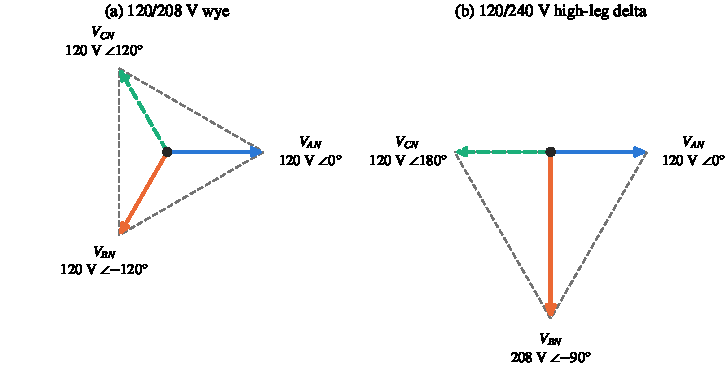
\includegraphics[width=0.85\linewidth]{figures/wye-vs-hl-phasor.pdf}
  \caption{Line-to-neutral phasors of (a) a 120/208\,V wye and (b) a 120/240\,V
    high-leg delta. In the wye all three are \SI{120}{\volt} and \ang{120} apart;
    in the delta, A and C are \ang{180} apart and B is \SI{208}{\volt} at
    \ang{90} to both.}
  \label{fig:wye-vs-hl}
\end{figure}

The same magnitude follows from geometry alone. B, N and A form a right-angled
triangle with the right angle at N: the hypotenuse B--A is one side of the delta,
\SI{240}{\volt}, and N--A is half the A--C winding, \SI{120}{\volt}. Hence
$|V_{BN}| = \sqrt{240^2 - 120^2} = \sqrt{43\,200} = 120\sqrt{3}\approx\SI{207.85}{\volt}$,
which agrees with \cref{eq:vbn}. \Cref{fig:hl-phasor} shows the construction,
and \cref{tab:hl-phasors} collects the results.

\begin{figure}[!h]
  \centering
  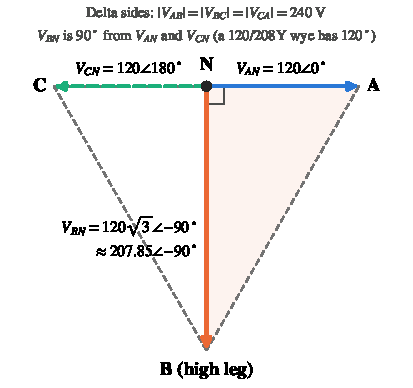
\includegraphics[width=0.6\linewidth]{figures/hl-phasor.pdf}
  \caption{Voltage phasors of a 120/240\,V centre-tapped closed delta, referenced
    to $V_{AN}$. The shaded B--N--A triangle gives $|V_{BN}| = \sqrt{240^2-120^2}
    = 120\sqrt{3}$\,V.}
  \label{fig:hl-phasor}
\end{figure}

\begin{table}[htbp]
  \centering
  \caption{Voltage phasors of a 120/240\,V centre-tapped closed delta,
    referenced to $V_{AN}$.}
  \label{tab:hl-phasors}
  \begin{tabular}{lll}
    \toprule
    Voltage  & Phasor               & Note \\
    \midrule
    $V_{AN}$ & $\ph{120}{0}$        & reference \\
    $V_{CN}$ & $\ph{120}{180}$      & reversed half of the A--C winding \\
    $V_{BN}$ & $\ph{207.85}{-90}$   & high leg, $120\sqrt{3}$\,V \\
    $V_{AB}$ & $\ph{240}{60}$       & \\
    $V_{BC}$ & $\ph{240}{-60}$      & lags $V_{AB}$ by \ang{120} \\
    $V_{CA}$ & $\ph{240}{180}$      & leads $V_{AB}$ by \ang{120} \\
    \bottomrule
  \end{tabular}
\end{table}

\begin{figure}[!h]
  \centering
  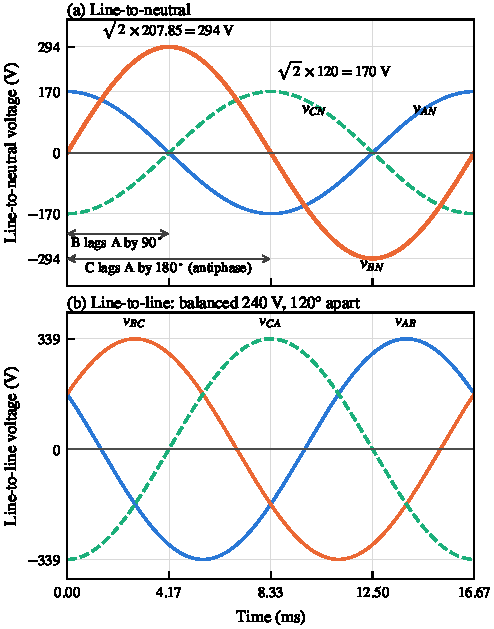
\includegraphics[width=0.6\linewidth]{figures/hl-waveforms.pdf}
  \caption{One cycle at \SI{60}{\hertz}. (a) Line-to-neutral: $v_{AN}$ and
    $v_{CN}$ are in antiphase with \SI{170}{\volt} peaks; $v_{BN}$ peaks at
    \SI{294}{\volt} and lags $v_{AN}$ by \ang{90}. (b) Line-to-line: a balanced
    240\,V set, \SI{339}{\volt} peak, \ang{120} apart.}
  \label{fig:hl-waveforms}
\end{figure}

% Example of the equation style, delete when you start:
% \begin{equation}
%   V_{BN} = \dots
%   \label{eq:vbn}
% \end{equation}

\subsection{Line currents for each kind of load}
\plan{120\,V loads (A--N, C--N); 240\,V two-pole loads on each pair; three-pole loads; superposition for a whole panel.}
\subsection{Why ``phase VA $\div$ 120'' fails}
\plan{Three-pole loads on 240\,V delta: +15.5\,\%. Two-pole loads on 120/208Y: $-13.3$\,\%. Two-pole loads on 240\,V delta: exact. Golden values in the repo: \texttt{data/golden/headline\_errors.csv}.}
\subsection{Phasor sum vs magnitude sum}
\subsection{Neutral current}
\subsection{Loading the utility bank}
\subsection{Voltage unbalance definitions}

% ---------------------------------------------------------------------
\section{Open delta}\label{sec:open-delta}
\status{outline, drafting in v0.3}
\subsection{Configurations}
\subsection{Capacity}
\plan{Derive the 57.7\,\% and 86.6\,\% figures.}
\subsection{Mixed single-phase and three-phase loading}
\subsection{Inherent voltage unbalance}
\subsection{Motors and drives on open delta}
\subsection{Failure modes}
\subsection{When to ask for a closed bank}

% =====================================================================
% PART II: THE 208 V QUESTION
% =====================================================================
\section{The 208\,V question}\label{sec:208v}
\status{outline, evidence collection now, drafting in v0.2}
\subsection{Two different ``208\,V'' problems}
\plan{Problem A: anything connected from the high leg to neutral. Problem B: 208\,V-rated equipment on a 240\,V service, and the reverse.}
\subsection{Method}
\plan{Evidence hierarchy: code text, standards, manufacturers, textbooks, utility rules, trade press, forums (practice evidence only). Record searches so the survey can be repeated.}
\subsection{Problem A: the high leg to neutral}
\subsection{Problem B: 208\,V and 240\,V equipment ratings}
\plan{Resistive loads scale with $V^2$: $(240/208)^2 \approx 1.33$. Motors and nameplate tolerance. Electronics.}
\subsection{Recommendations}

% =====================================================================
% PART III: WORKED EXAMPLES
% =====================================================================
\section{Worked example: a casual-dining restaurant}\label{sec:restaurant}
\status{base case agreed, drafting in v0.3}
\plan{Base case in the repo under \texttt{examples/restaurant/}. Load schedule; panel schedules (main, kitchen, front of house via 240$\Delta$--120/208Y transformer); exact vs shortcut currents; kitchen demand (candidates 220.56, 220.88); utility bank sizing; rebalancing; 208/240\,V rating checks; labels.}

\section{Worked example: a \SI{250}{m^3/day} SWRO plant on open delta}\label{sec:swro}
\status{base case agreed, drafting in v0.3}
\plan{Benchmarks \citep{infield2002swro}. Load schedule; motor circuits (candidates 430.250, 430.24); drives; open-delta bank sizing; unbalance at the motors; loss of one transformer; closed-bank comparison.}

% =====================================================================
% PART IV: IN THE FIELD
% =====================================================================
\section{Common issues and unforeseen circumstances}\label{sec:issues}
\status{outline, drafting in v0.4}
\plan{For each: symptom, cause, how to check, fix, prevention. Single-pole loads on the high leg; slash-rated breakers; SPDs and meters rated L--N; single-phase-input equipment on the high leg; PV and battery inverters; generators and transfer switches; loss of one open-delta transformer; motor unbalance; meter-base vs panelboard phase positions; utility conversion; 115/230\,V, 50\,Hz and imported equipment.}

\section{Waveforms and measurement}\label{sec:waveforms}
\status{outline, drafting in v0.4}
\plan{No field captures in this edition: every waveform is simulated or proxied and labelled.}

\section{The Caribbean context}\label{sec:caribbean}
\status{outline, drafting in v0.5}
\plan{Supply arrangements (researched and cited); 115/230\,V nominal; imported equipment; which code applies.}

\section{Validation}\label{sec:validation}
\status{outline, drafting in v0.5}
\plan{OpenDSS models; the IEEE Four-Wire Delta Test Feeder as benchmark; hand vs workbook vs Python vs OpenDSS.}

% =====================================================================
\bibliographystyle{unsrtnat}
\nocite{*}
\bibliography{refs}

% =====================================================================
\appendix
\section{Notation and formula sheet}\label{app:notation}
\status{filled in as \cref{sec:phasors} is drafted}

\section{Reproducing this note}\label{app:reproducing}
\plan{Layers: PDF; macro-free workbook; browser explorer; Python with uv; OpenDSS. Golden values in \texttt{data/golden/}.}

\section{Professional development mapping}\label{app:prof-dev}
\status{structure only}
\plan{CEng (UK-SPEC areas A--E) and BOETT criteria, once both are checked against current text.}

\section{Verification log}\label{app:verification}
\noindent\textit{Unverified}: candidate, not yet checked. \textit{Found}: located, not yet checked in full. \textit{Verified}: checked against the primary source (by whom, when).

\medskip
\noindent\begin{tabularx}{\linewidth}{@{}l l X l@{}}
\toprule
ID & NEC 2023 & Used for & Status \\
\midrule
C01 & 110.15 & High-leg marking & unverified \\
C02 & 230.56 & Service conductor with higher voltage to ground & unverified \\
C03 & 215.12, 210.5 & Feeder and branch identification & unverified \\
C04 & 408.3(E)(1) & Phase B arrangement & unverified \\
C05 & 408.3(F)(1) & High-leg field marking & unverified \\
C06 & 240.85 & Slash-rated breakers & unverified \\
C07 & 220.61 & Neutral load & unverified \\
C08 & Art.\ 242 & Surge protective devices & unverified \\
C09 & 220.56 & Kitchen equipment demand & unverified \\
C10 & 220.88 & Optional calculation, new restaurants & unverified \\
C11 & 430.250, 430.24 & Motor FLC; motor feeders & unverified \\
\bottomrule
\end{tabularx}

\medskip
\plan{External sources found so far (all ``found'', none verified): Moyer Diebel dishwasher listing (7.5\,kW at 208\,V vs 10.0\,kW at 240\,V); Infield (2002); Energy Recovery case studies; Fluke 1750 datasheet; Kersting (IEEE TIA); IEEE Four-Wire Delta Test Feeder; Mike Holt forum threads; Wikipedia ``High-leg delta'' (5\,\% claim, trace to source).}

\end{document}
